\documentclass[12pt]{article}
\def\x#1#2{$\mathbb{#1}^#2$} 
\def\n#1{\x#1}

\usepackage{graphicx}
\usepackage{latexsym}
\usepackage{amsfonts}
\usepackage{listings}
\usepackage{mypriptrt}
\usepackage{subfigure}
\usepackage{epic}


\title{NC LU - Abgabe 2} 
\author{Kern, Weichselbaum}

\abstract{
	Documentation for the first exercise of Neural Computation LU, Group 8.
}
\begin{document}
	
\maketitle	

\section{Einführung}

Die abgegebenen Dateien sind: calc_bias.m, calculate_weights.m, circle.m, draw_plot.m, draw_plot_rbf.m, genData.m, genDataRbf.m, generate_random_data.m, paintTraining.m, predictSVM.m, predictSVMRbf.m, predictSVMRbfws.m, rbfkernel.m, run.m, run_rbf.m, trainSVM.m, trainSVMRbf.m.
\\
\\
Zum Laufen wird das Ganze durch run.m gebracht. Diese Funktion hat keine Parameter und exekutiert den Code fuer 2.1, 2.2 und 2.3.

\section{SVM, Aufgabe 2}

Foo

\begin{figure}[htp]
	\centering
	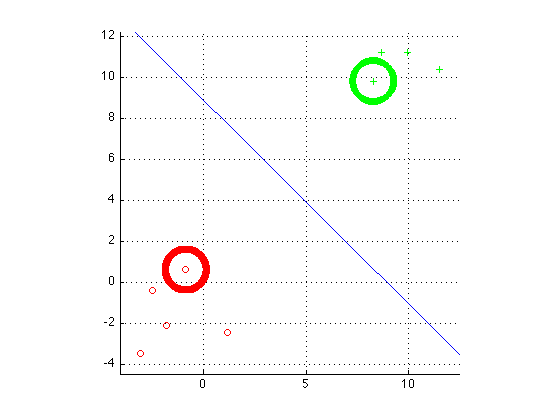
\includegraphics[width=1\textwidth]{linear_sep_data_plot}
	\caption{Datensatz, linear seperierbar, geplottet in Matlab. + ist Klasse 1, o signalisiert Klasse -1. Vektoren mit einem Kreis zeigen die Supportvektoren. Die Hyperplane ist optimal, da der Margin zwischen den Supportvektoren maximal ist.}
	\label{fig:linear_sep_data_plot}
\end{figure}
	
	
	
\begin{figure}[htp]
	\centering
	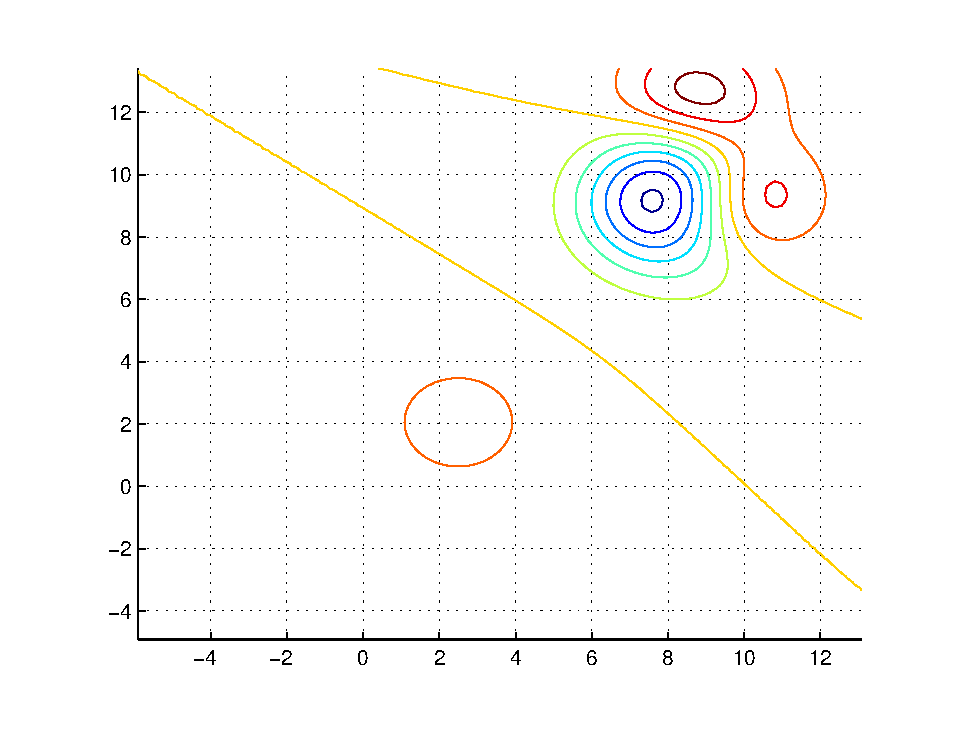
\includegraphics[width=1\textwidth]{contour}
	\caption{Datensatz, nicht linear seperierbar, mit contour in Matlab geplottet. Zeigt die Struktur des Datensatzes an Hand der gefunden Klassen.}
	\label{fig:contour}
\end{figure}

\end{document}


